%Diseño de Hardware
\section{Diseño de hardware} % (fold)
\label{sec:diseno_de_hardware}




Con el microcontrolador seleccionado, se procedió a la etapa de diseño de hardware. La placa de desarrollo C8051F350[\ref{sec:silicon_labs_c8051f352}] con la que se contó en el laboratorio donde se trabajo, sirvió de modelo para diseñar el circuito esquemático en la placa a desarrollar.

\subsection{Diagrama de Bloques de Hardware} % (fold)
\label{sub:diagrama_de_bloques_de_hardware}

La primera etapa de diseño consiste en diseñar un diagrama de bloques que ilustre a grandes rasgos la organización del circuito. Luego de esto se realiza el diseño esquemático que consiste en llevar cada bloque a nivel de componente electrónico y realizar la interconexión necesaria entre todos los elementos existentes para lograr el funcionamiento buscado. Los diagramas de bloque y esquemáticos se pueden ver en las figuras \ref{fig:bloquesHW} y \ref{fig:esquematico}. Con ayuda del software KiCad (\ref{sub:kicad}), se realizo el diagrama esquemático y la implementación en circuito impreso del esquemático construido.

\begin{figure}[h]
  \centering
  \includegraphics[width=0.80\textwidth, height = 9cm]{bloquesHW}
  \caption{\small Diagrama de bloques del circuito a realizar}\label{fig:bloquesHW}
\end{figure}

Los bloques en la figura \ref{fig:bloquesHW} representan de forma general los distintos módulos a implementar. Las entradas analógicas entran al sistema a través de filtros que reducen el ruido. Luego ingresan al microcontrolador para ser procesadas. El bloque de GPIO y contadores de eventos es simplemente un grupo de pines direccionados a distintas entradas del microcontrolador. GPIO significa ``General Purpose Input Output''( en español, ``entrada y salida de propósito general'' ). Son 4 pines que se separaron para uso general, por necesidad eventual de necesitarlos. Parte de estos GPIO son los pines contadores de eventos, por lo cual se incluyeron dentro del mismo bloque.

Es posible alimentar el sistema por medio del programador, o mediante una tension de 3,3V que se obtiene como salida de un regulador de tension, cuya entrada es de 5V. La llave selectora decide si se alimenta el sistema usando la alimentación por fuente continua de 5V, o por el programador.

% subsection diagrama_de_bloques_de_hardware (end)



\subsection{Diagrama Esquemático} % (fold)
\label{sub:diagrama_esquematico}

La figura \ref{fig:esquematico} muestra el diagrama esquemático del circuito a implementar. El microcontrolador[\ref{sec:silicon_labs_c8051f352}] con el que se trabaja tiene ciertos niveles de tension de operación con el que se trabaja. En principio, se alimenta con una fuente de 5V y 500mA que trabaja junto con un regulador de tension[\cite{bib:lm2937}] que lleve la alimentación a un nivel de 3,3V. Estos 3,3V se utilizan para alimentar al microcontrolador; la tension analógica positiva del conversor; a un integrado MAX232[\cite{bib:max232}] que se utiliza para lograr una interfaz serial entre la UART[\ref{sub:interfaz_serial}] de la placa y un puerto serial de una PC; y a un led testigo de alimentación.

\begin{figure}[h]
  \centering
  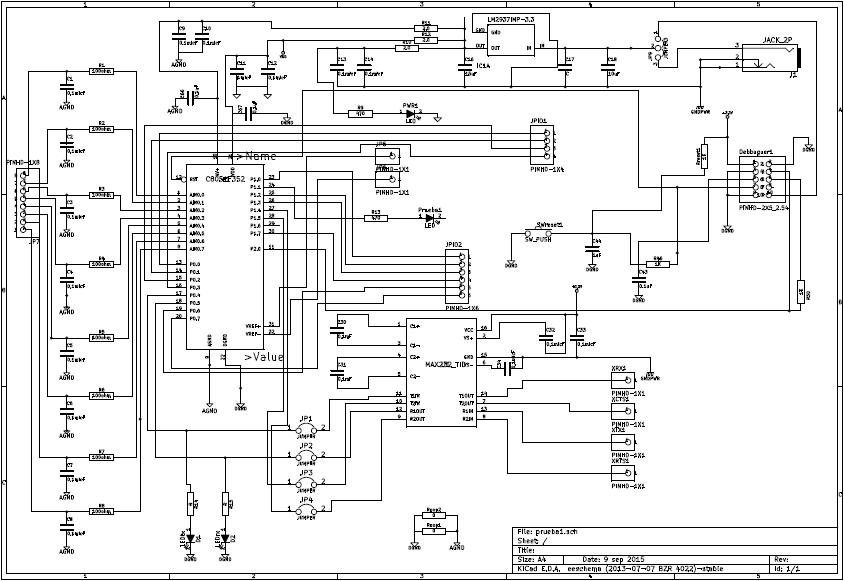
\includegraphics[width=0.95\textwidth, height = 10cm]{esquematico}
  \caption{\small Diagrama esquemático del circuito realizado}\label{fig:esquematico}
\end{figure}


% subsection diagrama_esquemático (end)

\subsection{Implementación en Circuito Impreso} % (fold)
\label{sub:implementacion_en_circuito_impreso}

Una implementación en circuito impreso consiste simplemente en pasar de un diagrama esquemático al despliegue físico de los componentes reales en una PCB (en inglés, Printed Circuit Board). Para esto, se utilizaron funcionalidades del software KiCad, que también se utilizo para realizar el esquemático del circuito. Una imagen del resultado del despliegue de componentes esta en la figura \ref{fig:PCB1}.

\begin{figure}[h]
  \centering
  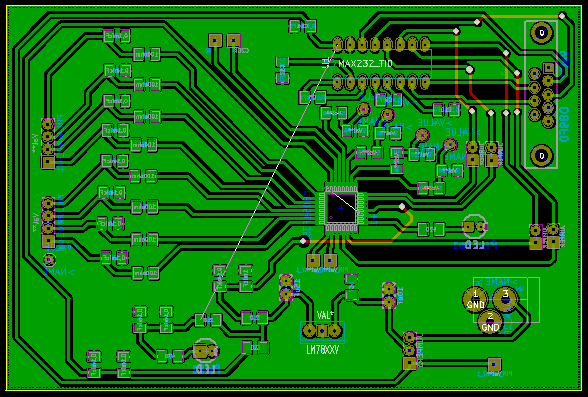
\includegraphics[width=0.95\textwidth, height = 10cm]{PCB1}
  \caption{\small Diagrama del despliegue de componentes}\label{fig:PCB1}
\end{figure}

% subsection implementación_en_circuito_impreso (end)

\subsection{Circuito anexo de programación} % (fold)
\label{sub:circuito_anexo_de_programacion}

Para programar el microcontrolador, se utiliza un programador de la marca de Silicon Labs hecho para la placa de desarrollo utilizada. Es posible usar este mismo programador en la plataforma a construir, pero es necesario armar un circuito que funcione como interfaz entre la placa del microcontrolador y el programador de la misma. El circuito se muestra en la figura \ref{fig:PCB2}.

\begin{figure}[H]
  \centering
  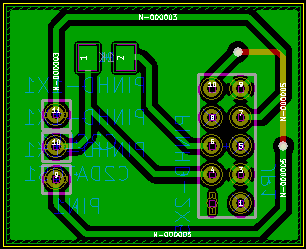
\includegraphics[width=0.20\textwidth, height = 3cm]{PCB2}
  \caption{\small Diagrama del despliegue de componentes del circuito que hace de interfaz entre el programador y la plataforma}\label{fig:PCB2}
\end{figure}

% subsection circuito_anexo_de_programación (end)

\subsection{Impresión del circuito en placa de cobre} % (fold)
\label{sub:impresion_del_circuito_en_placa_de_cobre}

La impresión de la placa física se implemento mas de una vez, hasta que fue posible correr un programa en el sistema y verificar su funcionamiento. Hubo cuatro versiones en total. En cada una de ellas salieron a la vista distintos errores que hacian necesaria una nueva impresion para corregirlos.

\begin{figure}[h]
  \centering
  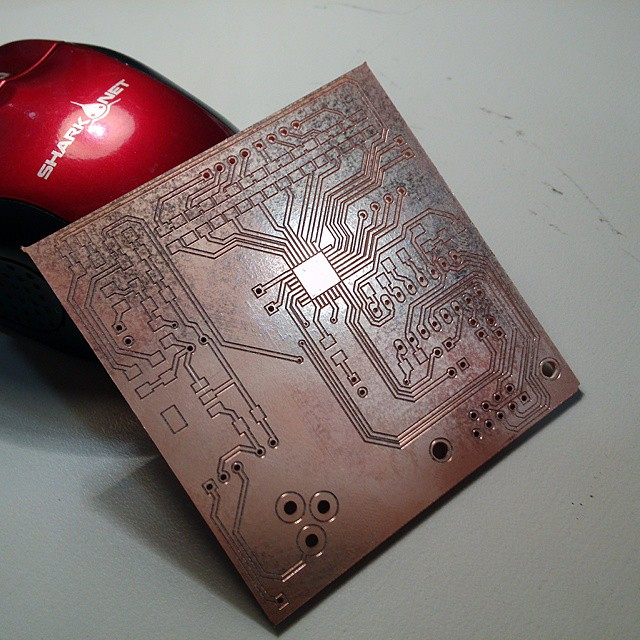
\includegraphics[width=0.95\textwidth, height = 10cm]{placa1}
  \caption{\small Fotografia del primer prototipo}\label{fig:placa1}
\end{figure}

La primera version de la placa se puede ver en la figura \ref{fig:placa1}. En esta primera placa hubo errores de diseño del despliegue de componentes, ya que varias de las pistas se solapaban, y esto hubiese provocado cortocircuito entre las pistas.

\begin{figure}[h]
  \centering
  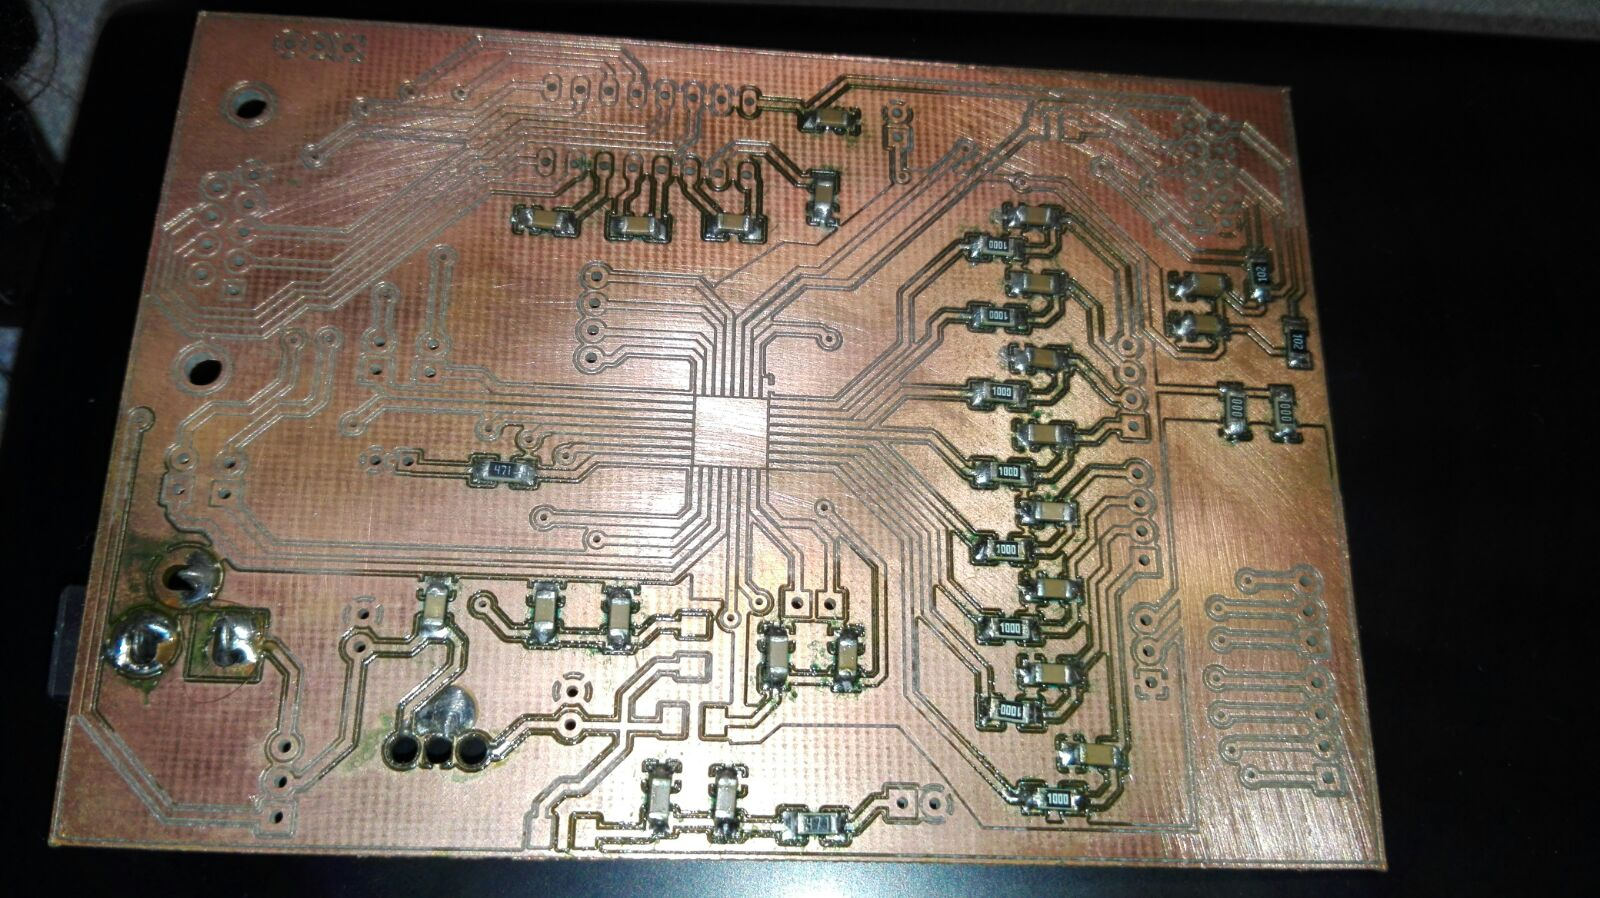
\includegraphics[width=0.95\textwidth, height = 10cm]{placa2}
  \caption{\small Fotografia del segundo prototipo}\label{fig:placa2}
\end{figure}

En la segunda version se experimentaron problemas relacionados al ancho de los huecos de las patas de algunos componentes. En particular, el encapsulado del regulador de tension de 3,3V, encargado de suministrar tension al microcontrolador, no podia colocarse correctamente en la placa. Al ser una pieza tan importante, dado que sin el el microcontrolador no enciende, hubo que rehacer la placa[\cite{bib:lm2937}]

\begin{figure}[h]
  \centering
  \includegraphics[width=0.95\textwidth, height = 10cm]{placa3}
  \caption{\small Fotografia del tercer prototipo}\label{fig:placa3}
\end{figure}



\begin{figure}[h]
  \centering
  \includegraphics[width=0.95\textwidth, height = 10cm]{placa4}
  \caption{\small Fotografia del cuarto y ultimo prototipo}\label{fig:placa4}
\end{figure}



% subsection impresión_del_circuito_en_placa_de_cobre (end)

% section diseño_de_hardware (end)